\subsection{Necessidade de Desenho de Software Resiliente}\label{subsec:necessidade-de-desenho-de-software-resiliente}
A utilização de sistemas distribuídos é cada vez mais preponderante nos tempos atuais.
Estes sistemas representam um conjunto de computadores independentes e interligados em rede, que se apresentam aos utilizadores como um sistema único e coerente~\cite{fcc-distributed-systems}.

Dado a constante necessidade destes sistemas estarem disponíveis, aliados à sua complexidade de funcionamento, é natural que estejam suscetíveis a falhas de comunicação, de hardware, de software, entre outras.
Por esse motivo, existe a necessidade de garantir que os serviços que disponibilizam sejam resilientes, e mais concretamente, tolerantes a falhas.

Um serviço tolerante a falhas, é um serviço que é capaz de manter a sua funcionalidade total ou parcial, ou apresentar uma alternativa, quando um ou mais componentes que lhes estão associados falham.
De forma a alcançar este objetivo, foram desenhadas estratégias de resiliência.
Alguns exemplos são:

\begin{itemize}[topsep=0pt,itemsep=0pt,partopsep=0pt, parsep=0pt]
    \item \textbf{Retry}: Tenta novamente uma operação que falhou, aumentando a sua probabilidade de sucesso;
    \item \textbf{Rate Limiter}: Limita a taxa de requisições que um determinado serviço pode receber;
    \item \textbf{Circuit Breaker}: Interrompe, temporariamente, a comunicação com um serviço que está a falhar, de forma a evitar que o mesmo sobrecarregue o sistema. Semelhante a um disjuntor elétrico;
    \item \textbf{Fallback}: Fornece um valor ou executa uma ação alternativa caso uma operação falhe.
\end{itemize}

\subsection{Bibliotecas como Mecanismos de Resiliência}\label{subsec:bibliotecas-como-mecanismos-de-resiliencia}

Existem bibliotecas que atuam como mecanismos de resiliência (Tabela~\ref{tab:resilience_libraries}) e que disponibilizam estratégias, também designadas como \textit{policies}.
Estas podem ser configuradas consoante as necessidades do sistema e aplicadas a operações específicas, como por exemplo, a comunicação com um serviço externo.

\begin{table}[h]
    \centering
    \caption{Exemplos de bibliotecas como mecanismos de resiliência.}
    \label{tab:resilience_libraries}
    \begin{tabular}{|l|l|l|l|}
        \hline
        \textbf{Biblioteca}                      & \textbf{Linguagem} & \textbf{Plataforma} \\ \hline
        Netflix's Hystrix~\cite{netflix-hystrix} & Java               & JVM                 \\ \hline
        Resilience4j~\cite{resilience4j}         & Java/Kotlin        & JVM                 \\ \hline
        Polly ~\cite{polly-dotnet}               & C\#                & .NET                \\
        \hline
    \end{tabular}
\end{table}

A biblioteca Polly~\cite{polly-dotnet} divide as estratégias de resiliência em duas categorias:

\begin{itemize}[topsep=0pt,itemsep=0pt,partopsep=0pt, parsep=0pt]
    \item \textbf{Resiliência Reativa}: Reage a falhas e mitiga o seu impacto (e.g., \textit{Retry, Circuit Breaker});
    \item \textbf{Resiliência Proativa}: Previne que as falhas aconteçam (e.g., \textit{Rate Limiter, Timeout}).
\end{itemize}

\subsection{Kotlin Multiplatform}\label{subsec:kotlin-multiplatform}

A tecnologia \textit{Kotlin MultiPlatform}~\cite{kmp} (\textit{KMP}) possibilita a partilha do código da aplicação entre diversas plataformas.
A sua arquitetura (Figura~\ref{fig:kmp-architecture}) é composta por três categorias principais:

\begin{itemize}[topsep=0pt,itemsep=0pt,partopsep=0pt, parsep=0pt]
    \item \textbf{Common}: Código partilhado entre todas as plataformas (i.e., \textit{CommonMain, CommonTest});
    \item \textbf{Intermediary}: Código que pode ser partilhado num conjunto particular de plataformas;
    \item \textbf{Specific}: Código específico de uma plataforma-alvo (i.e., \textit{\textless Plataform\textgreater Main, \textless Plataform\textgreater Test}).
\end{itemize}

O objetivo principal é a maximização da reutilização de código, ou seja, agregar o máximo de código possível na categoria \textit{Common}.
No entanto, por vezes é necessário criar código específico para uma plataforma-alvo, regularmente denominada como \textit{target}, nas seguintes situações:

\begin{itemize}[topsep=0pt,itemsep=0pt,partopsep=0pt, parsep=0pt]
    \item Uma determinada funcionalidade não consegue ser implementada de forma comum porque:
    \begin{itemize}[topsep=0pt,itemsep=0pt,partopsep=0pt, parsep=0pt]
        \item é necessário acesso a API's especificas do \textit{target};
        \item as bibliotecas disponíveis para código comum (i.e., \textit{Standard Kotlin Library, Kotlinx}) não cobrem as funcionalidades pretendidas;
    \end{itemize}
    \item Um determinado \textit{target} não suporta diretamente o \textit{KMP} (e.g., \textit{Node.js)}, e por isso é necessário criar um \textit{adapter} para a comunicação com o código comum.
\end{itemize}

Para criar código específico para um \textit{target} é utilizado o
mecanismo \textbf{\textit{expect/actual}}~\cite{kmp-expect-actual}, que permite a definição do código a ser implementado e a sua implementação, respetivamente.

\begin{figure}[H]
    \centering
    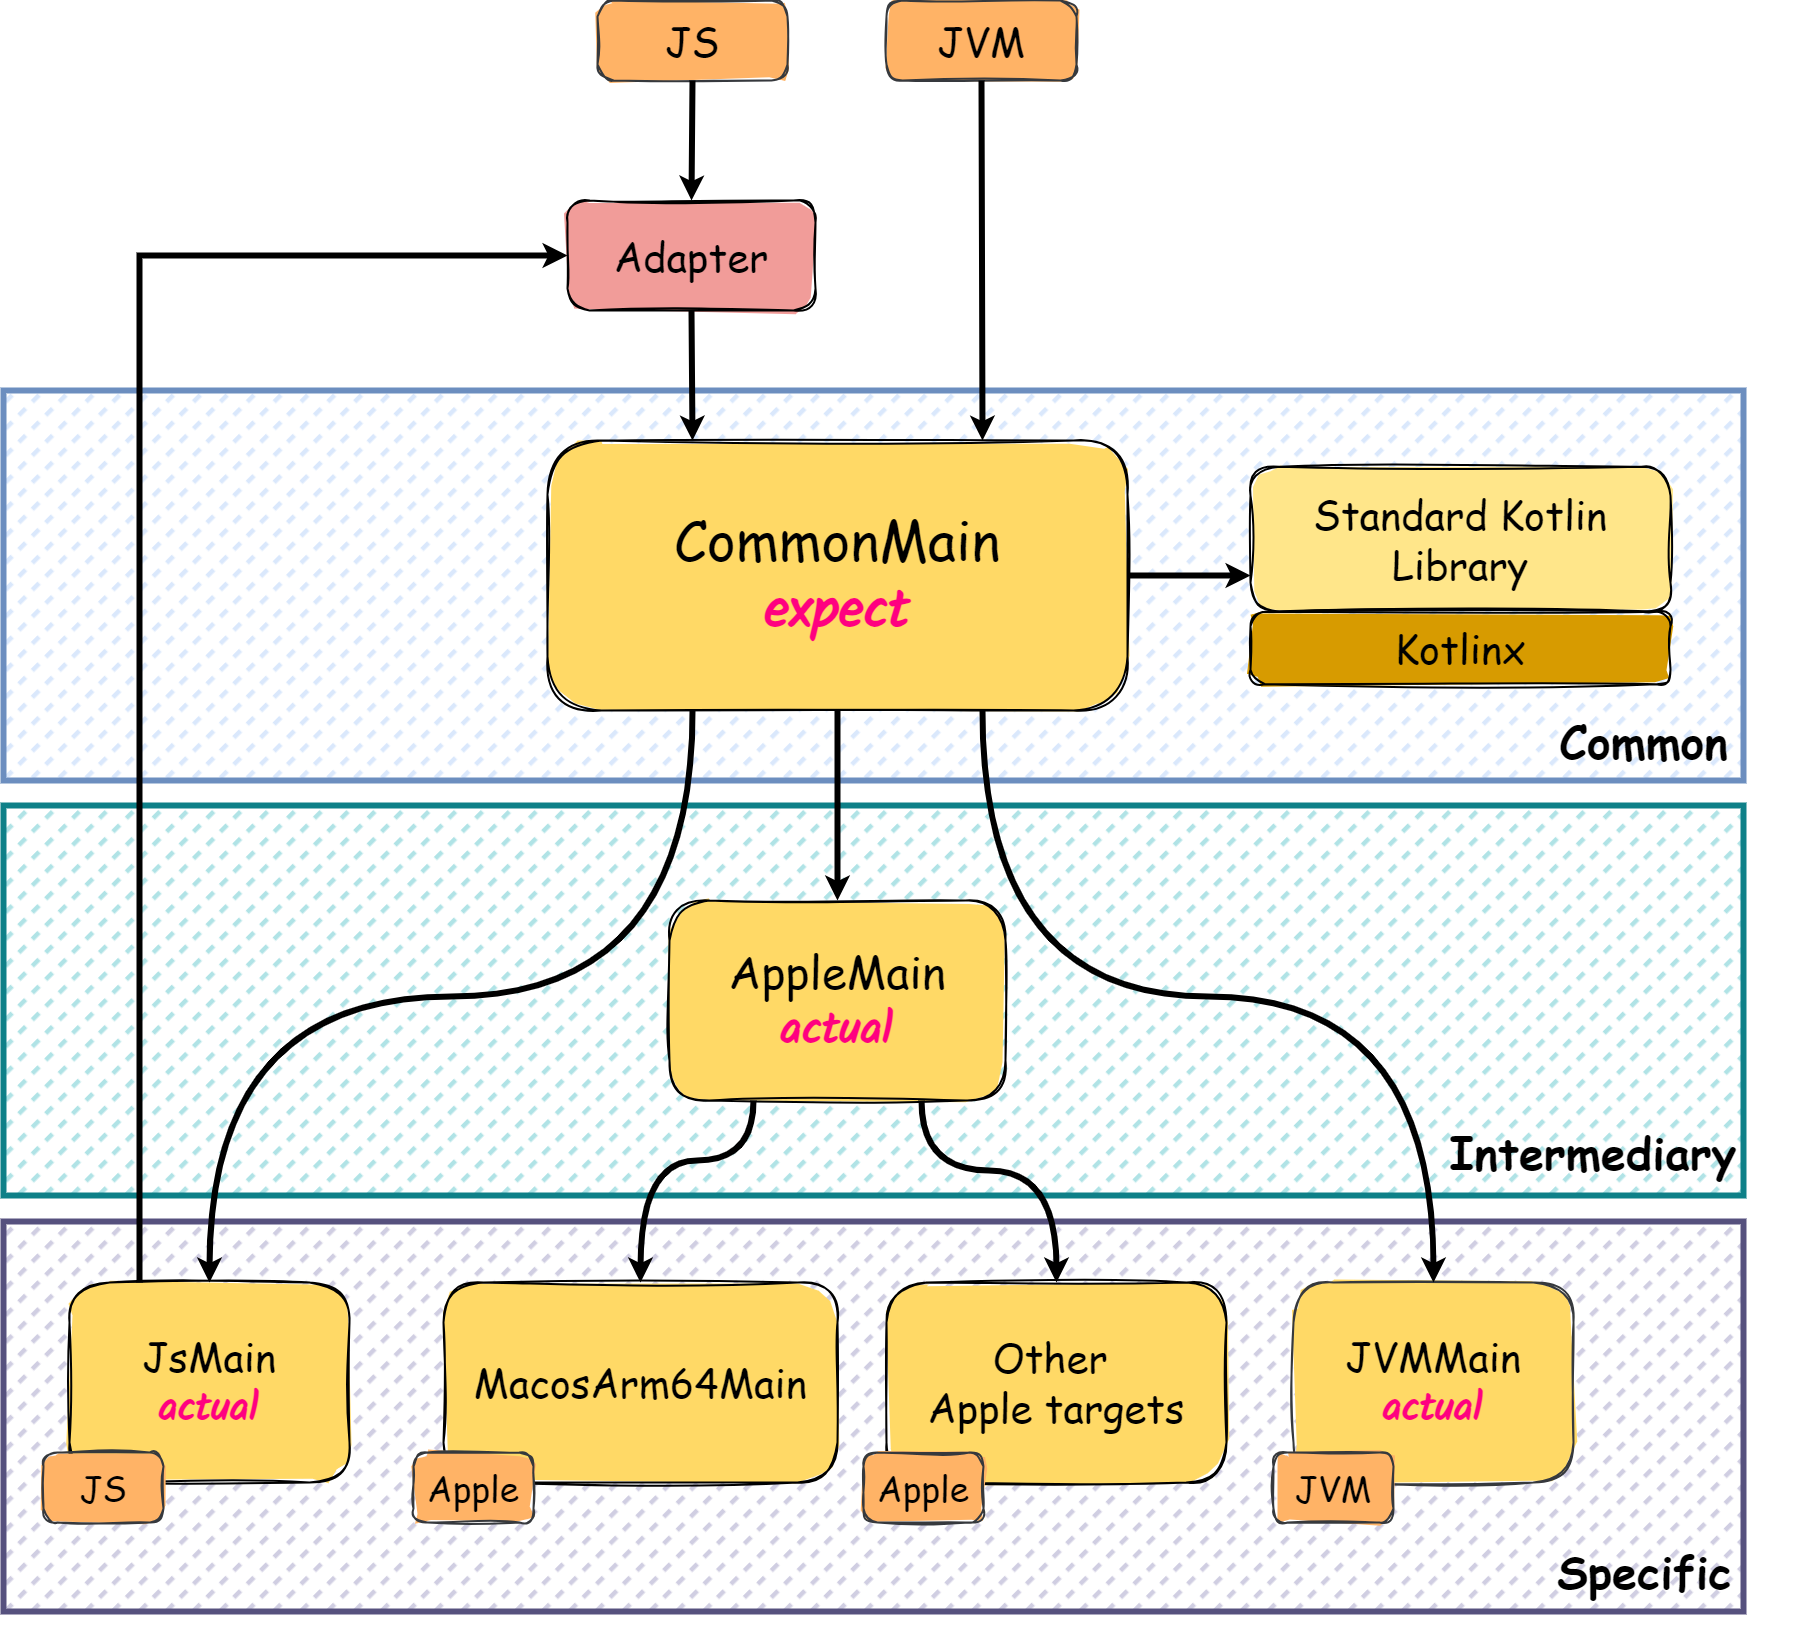
\includegraphics[width=0.5\textwidth]{../docs/imgs/kmp-architecture}
    \caption{Arquitetura do \textit{KMP}.}
    \label{fig:kmp-architecture}
\end{figure}

\subsection{Ktor}\label{subsec:ktor}

\textit{Ktor}~\cite{ktor} é uma framework \textit{KMP} modular para desenvolver aplicações assíncronas de
servidor e cliente. Desenvolvida pela \textit{JetBrains}, foi construída com \textit{Kotlin} puro e está integrada com o sistema de \textit{Coroutines}. Sistema esse que permite a definição de
código assíncrono de forma sequencial e a sua execução sem bloqueio de threads, tirando maior proveito do sistema computacional disponível.
